\documentclass[10pt, export]{beamer}

\usepackage[utf8]{inputenc}
\usepackage[T1]{fontenc}
    
\usepackage{standalone}
    
\usepackage[acronym]{glossaries}
    
\usepackage{enumitem}
    
\usepackage{xcolor}
    
\usepackage{multirow}
\usepackage{multicol}
    
\usepackage{array}
\newcolumntype{x}[1]{>{\centering\let\newline\\\arraybackslash\hspace{0pt}}p{#1}}
\usepackage{booktabs, colortbl}
    
\usepackage{siunitx}
\usepackage{mathrsfs, amsmath}
    
\usepackage{graphicx}
\usepackage{subcaption}
\usepackage[font={small, color=black}, labelformat=empty]{caption}
\DeclareCaptionFont{tiny}{\tiny}
\usepackage[font={tiny, color=black}, labelformat=empty]{subcaption}
\usepackage{adjustbox}

\usepackage{tikz}
\usetikzlibrary{calc}


\usepackage{pifont, textcomp}
\newcommand{\cmark}{{\color{green} \ding{51}}}%
\newcommand{\xmark}{{\color{red} \ding{55}}}%

\usepackage{colortbl}
\definecolor{Moins4}{RGB}{183,10,10}
\definecolor{Moins3}{RGB}{255,0,0}
\definecolor{Moins2}{RGB}{255,122,12}
\definecolor{Moins1}{RGB}{255,181,12}
\definecolor{Zero}{RGB}{255,255,255}
\definecolor{Plus1}{RGB}{58,255,12}
\definecolor{Plus2}{RGB}{58,155,12}


\usepackage{hyperref}

\usepackage[useregional]{datetime2}
    
\usepackage[
        mcite,
        backend=bibtex,
        style=verbose,
        citestyle=authoryear,
        bibstyle=numeric,
        sorting=none,
        autocite=footnote,
        maxnames=2,
        hyperref=true,
        natbib=true,
        abbreviate=true
    ]{biblatex}
\bibliography{references}
\setbeamerfont{footnote}{size=\tiny}


\usetheme{ign}


\newacronym{acr::lod}{LoD}{Level of Detail}
\newacronym{acr::elod}{eLoD}{evaluation Level of Detail}
\newacronym{acr::lidar}{LiDAR}{Light Detection and Ranging}
\newacronym{acr::dsm}{DSM}{Digital Surface Model}
\newacronym{acr::gui}{GUI}{Graphical User Interface}

\title{Reconstructed 3D building model evaluation}
\subtitle{the forgotten step}
\date{\tiny\DTMdisplaydate{2019}{4}{19}{5}}
\author{\scriptsize Oussama Ennafii \inst{1, 2}, Arnaud Le Bris \inst{1}, Cl\'ement Mallet \inst{1}, Florent Lafarge \inst{2}}
\institute{\scriptsize \inst{1} Univ. Paris Est, LaSTIG STRUDEL, IGN, ENSG\\ \scriptsize \inst{2} Inria, TITANE}

\begin{document}
    \begin{frame}[plain]
        \titlepage{}
    \end{frame}

    \section{Introduction}
        \begin{frame}{Context: 3D model vs. 3D mesh}
            \begin{figure}
                \begin{center}
                    \begin{subfigure}{\textwidth}
                        \begin{center}
                            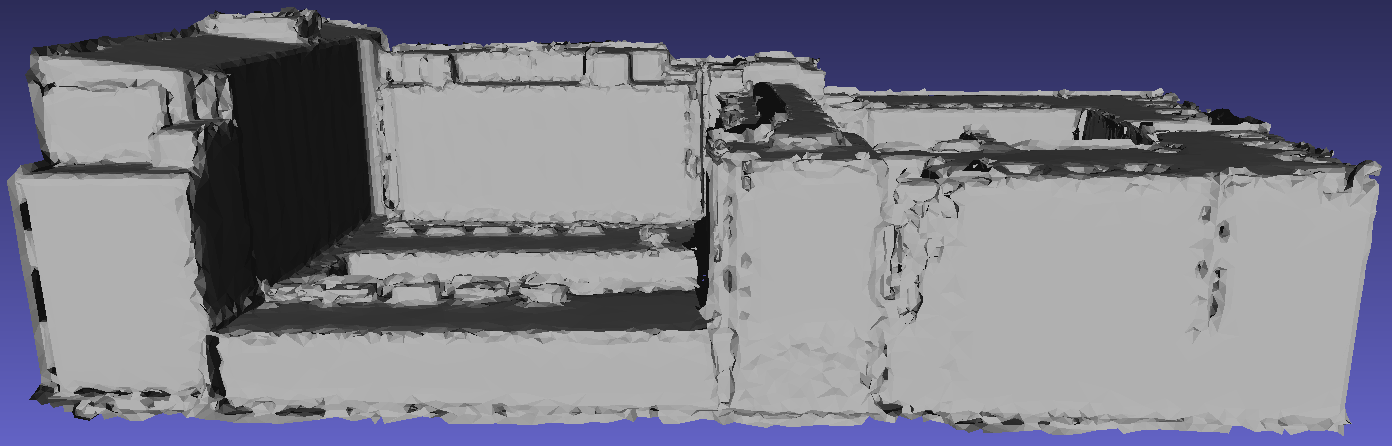
\includegraphics[height=.28\textheight]{images/difference_mesh_model/bercy_building_mesh_1_e5}
                            \caption{\small 3D mesh of a building surface ($\approx$ \num[output-exponent-marker = \text{e}]{1e5} triangles).}
                        \end{center}
                    \end{subfigure}
                    \\
                    \begin{subfigure}{\textwidth}
                        \begin{center}
                            \includestandalone[mode=buildnew, height=.28\textheight]{ground_truth_model}
                            \caption{\small Building 3D polyhedral model ($\approx$ 800 facets).}
                        \end{center}
                    \end{subfigure}
                    \caption{Different model schemes of a building ($\approx$ \SI{139 x 71 x 23}{\metre}).}
                \end{center}
            \end{figure}
        \end{frame}
        \begin{frame}{Motivation}
            \only<1-4>{
                \begin{itemize}[label=$\blacktriangleright$, font=\color{IGNGreen}, itemsep=2em]
                    \item<1-> Automatic urban modeling: an active research area~\citep{Musialski2012};
                    \item<2-> Results seamless but lack generality and often erroneous~\citep{rottensteiner2014results};
                    \begin{itemize}[label=$\longrightarrow$]
                        \item<3-> labourious manual corrections.
                    \end{itemize}
                    \item<4-> Urban 3D model semantic diagnostic \textcolor{purple}{not well studied}~\citep{nguatem2017modeling};
                \end{itemize}
            }
            \only<5->{
                \begin{itemize}[label=Goal $\longrightarrow$, font=\color{purple}, leftmargin=2cm]
                    \item<5-> Detect and describe semantic errors that affect building 3D models.
                \end{itemize}
                \begin{itemize}[label=$\blacktriangleright$, font=\color{IGNGreen}, itemsep=2em]
                    \item<6-> Semantic errors independent from \textbf{reconstruction methods} and \textbf{urban scenes}.
                    \item<7-> \textbf{Transferability}, and hence scalability, of the evaluation method.
                \end{itemize}
            }
        \end{frame}
        \begin{frame}{Potential use}
            \begin{itemize}[label=$\blacktriangleright$, font=\color{IGNGreen}, itemsep=2em]
                \item<1-> Change detection;
                \item<2-> Urban models correction;
                \item<3-> Urban reconstruction method evaluation;
                \item<4-> Crowd reconstruction quality assessment.
            \end{itemize}
        \end{frame}

    \section{Methodology}
            \begin{frame}{Main ideas behind our approach}
                \begin{itemize}[label=$\blacktriangleright$, font=\color{IGNGreen}, itemsep=2em]
                    \item<1-> Compile errors that affect building models in a taxonomy;
                    \item<2-> Evaluation at building level $\Longrightarrow$ formulated as a supervised classification problem;
                    \item<3-> Study in a \textbf{2.5D overhead (aerial)} modeling setting.
                \end{itemize}
            \end{frame}
            \subsection{Error taxonomy}
            \begin{frame}{Taxonomy structure}
                Two criteria determine the taxonomy structure:
                \begin{itemize}[label=$\blacktriangleright$, font=\color{IGNGreen}, itemsep=2em]
                    \item<2-> the \textbf{\acrfull{acr::lod}};
                    \item<3-> the \textbf{\texttt{finesse}}: the semantic evaluation level.
                \end{itemize}
                ~\\
                \uncover<4->{
                    \begin{block}{Definition}
                        error of maximal \texttt{finesse} $\Leftrightarrow$ corresponds \textit{semantically} to a \textit{unitary} action required to correct the model $\Leftrightarrow$ \texttt{atomic}.
                    \end{block}
                }
            \end{frame}
            \begin{frame}{\acrshort{acr::lod}: a brief reminder}
                \begin{figure}
                    \begin{center}
                        \includestandalone[mode=buildnew, width=\textwidth]{lods}
                    \end{center}
                    \caption{Basic \acrshort{acr::lod} classification used in Computer Vision.}
                \end{figure}
            \end{frame}    
            \begin{frame}{Error taxonomy (\texttt{finesse} $= 0$)}
                \begin{figure}
                    \includestandalone[mode=buildnew, width=\textwidth]{finesse_0_taxonomy}
                \end{figure}
            \end{frame}
            \begin{frame}{Error taxonomy (\texttt{finesse} $= 1$)}
                \begin{figure}
                    \includestandalone[mode=buildnew, width=\textwidth]{finesse_1_taxonomy}
                \end{figure}
            \end{frame}
            \begin{frame}{Error taxonomy (\texttt{finesse} $= 2$)}
                \only<1>{
                    \begin{figure}
                        \includestandalone[mode=buildnew, width=\textwidth]{finesse_2_taxonomy}
                    \end{figure}
                }
                \only<2>{
                    \begin{figure}
                        \includestandalone[mode=buildnew, width=\textwidth]{finesse_2_taxonomy_lods}
                    \end{figure}
                }
            \end{frame}
            \begin{frame}{Error taxonomy (\texttt{finesse} $= 3$, $\leq$ \acrshort{acr::lod}-1)}
                \begin{figure}
                    \includestandalone[mode=buildnew, width=\textwidth]{finesse_3_bul_taxonomy}
                \end{figure}
            \end{frame}
            \begin{frame}{Building \texttt{atomic} errors: 2.5D overhead reconstruction case}
                \only<1>{
                    \begin{figure}
                        \begin{center}
                            \begin{subfigure}{.4\textwidth}
                                \centering
                                \fbox{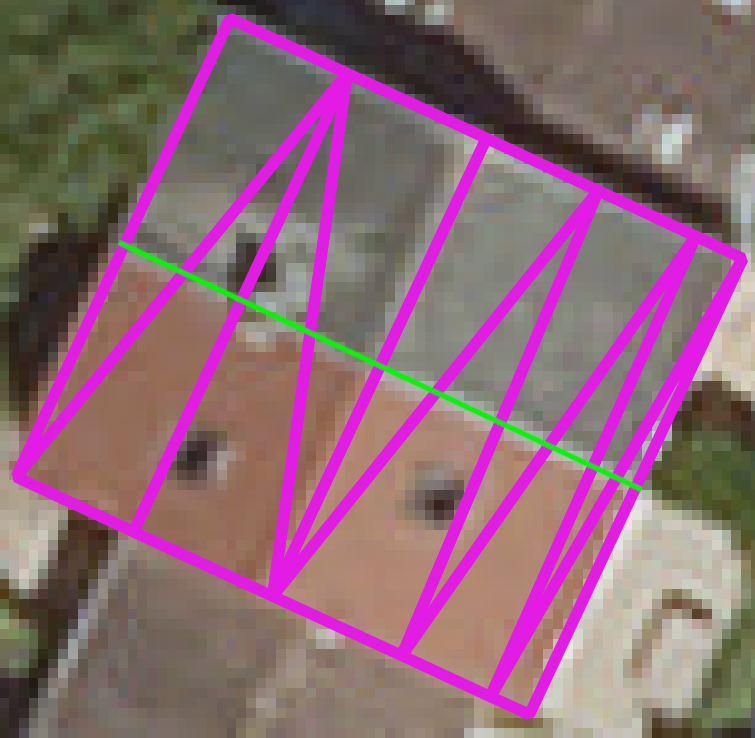
\includegraphics[height=.45\textheight]{images/errors/building/under_segmentation}}
                                \caption{\label{fig::bul_under} Under segmentation (\texttt{BUS}).}
                            \end{subfigure}
                            \begin{subfigure}{.5\textwidth}
                                \centering
                                \fbox{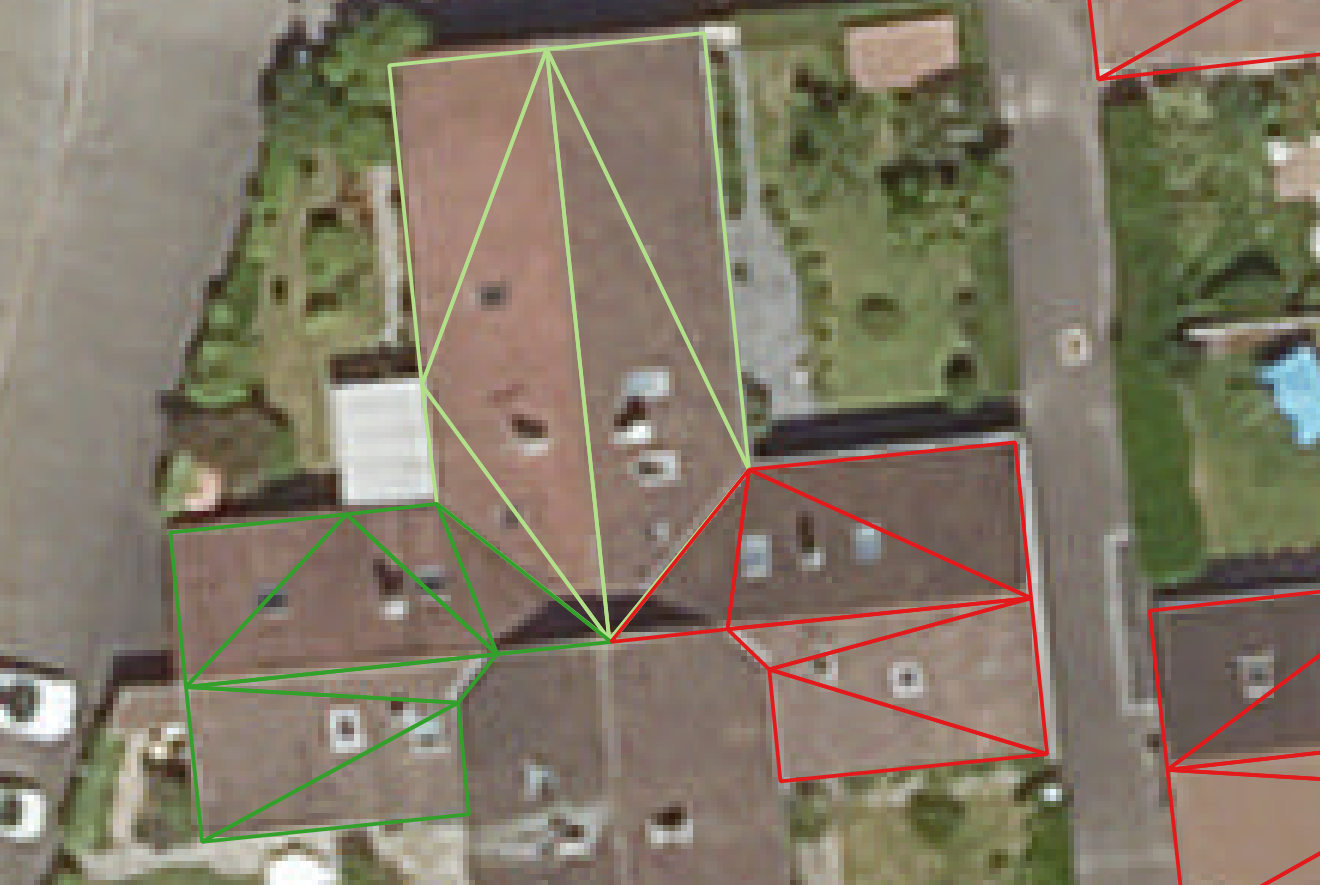
\includegraphics[height=.45\textheight]{images/errors/building/over_segmentation}}
                                \caption{\label{fig::bul_over} Over segmentation (\texttt{BOS}).}
                            \end{subfigure}
                        \end{center}
                    \end{figure}
                }
                \only<2>{
                    \begin{figure}
                        \begin{center}
                            \begin{subfigure}{.45\textwidth}
                                \centering
                                \fbox{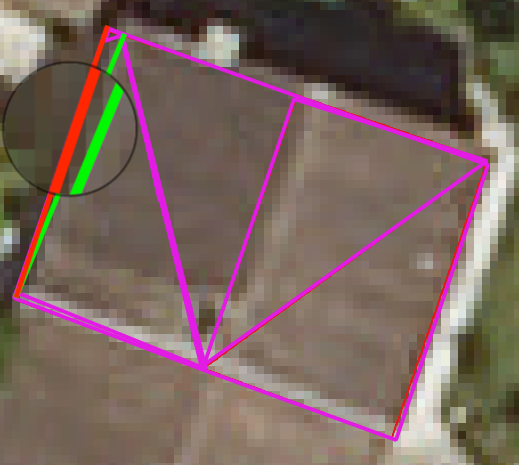
\includegraphics[height=.5\textheight]{images/errors/building/border}}
                                \caption{\label{fig::bul_footprint} Imprecise border (\texttt{BIB}).}
                            \end{subfigure}
                            \begin{subfigure}{.45\textwidth}
                                \centering
                                \fbox{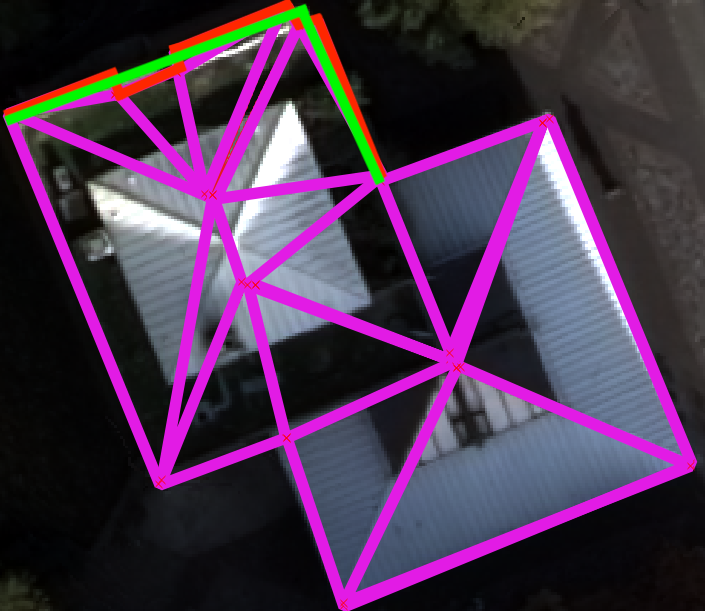
\includegraphics[height=.5\textheight]{images/errors/building/topology}}
                                \caption{\label{fig::bul_height} Inaccurate topology (\texttt{BIT}).}
                            \end{subfigure}
                        \end{center}
                    \end{figure}
                }
            \end{frame}
            \begin{frame}{Error taxonomy (\texttt{finesse} $= 3$, $\leq$ \acrshort{acr::lod}-2)}
                \begin{figure}
                    \includestandalone[mode=buildnew, width=\textwidth]{finesse_3_all_taxonomy}
                \end{figure}
            \end{frame}
            \begin{frame}{Facet \texttt{atomic} errors: 2.5D overhead reconstruction case}
                \only<1>{
                    \begin{figure}
                        \begin{center}
                            \begin{subfigure}{.26\textwidth}
                                \centering
                                \fbox{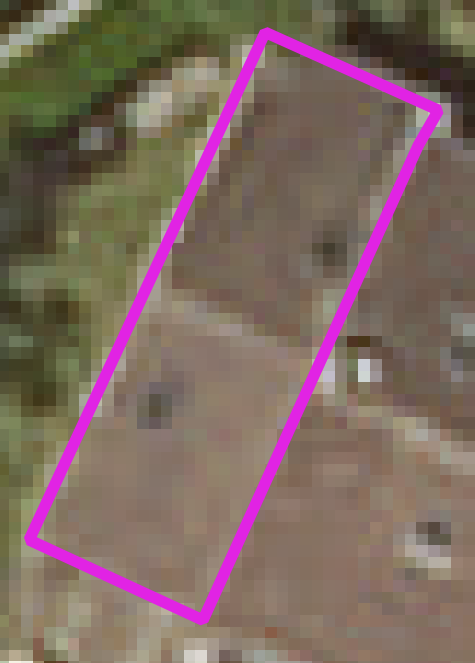
\includegraphics[height=.4\textheight]{images/errors/facet/under_segmentation}}
                                \caption{\label{fig::fac_under} Under segmentation}
                            \end{subfigure}
                            \begin{subfigure}{.31\textwidth}
                                \centering
                                \fbox{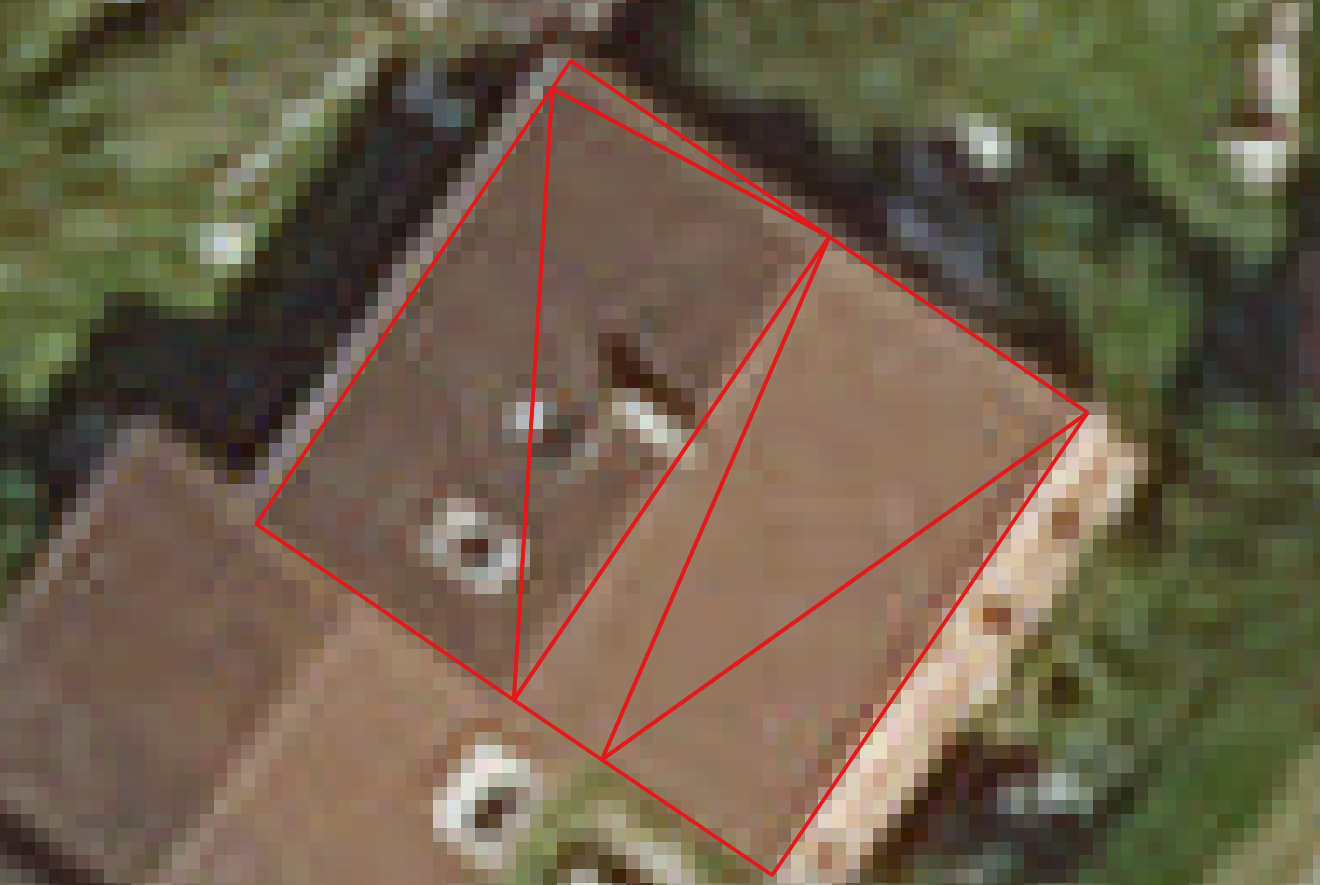
\includegraphics[height=.4\textheight]{images/errors/facet/over_segmentation}}
                                \caption{\label{fig::fac_over} Over segmentation}
                            \end{subfigure}
                            \begin{subfigure}{.37\textwidth}
                                \centering
                                \fbox{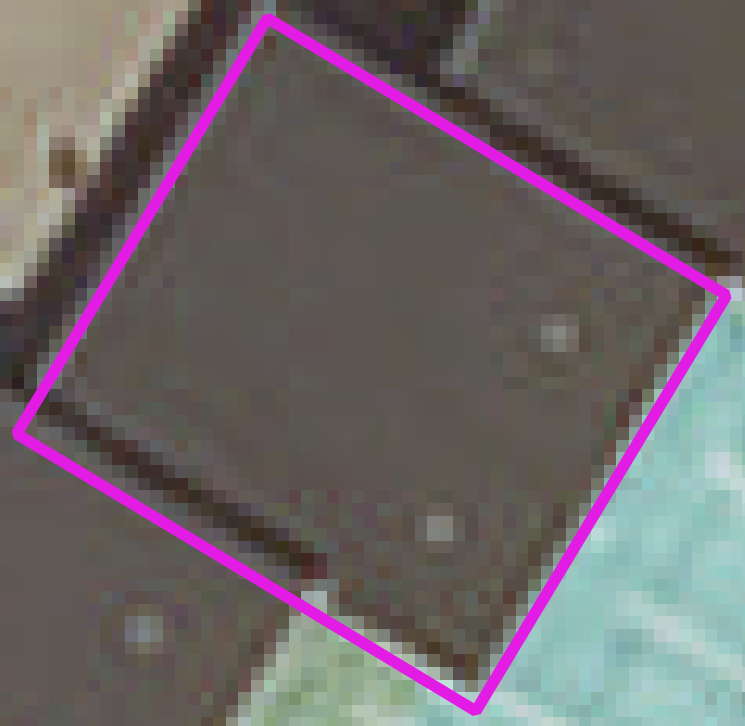
\includegraphics[height=.4\textheight]{images/errors/facet/geometry}}
                                \caption{\label{fig::fac_height} Imprecise geometry}
                            \end{subfigure}
                        \end{center}
                    \end{figure}
                }
                \only<2>{
                    \begin{figure}
                        \begin{center}
                            \begin{subfigure}{.45\textwidth}
                                \centering
                                \fbox{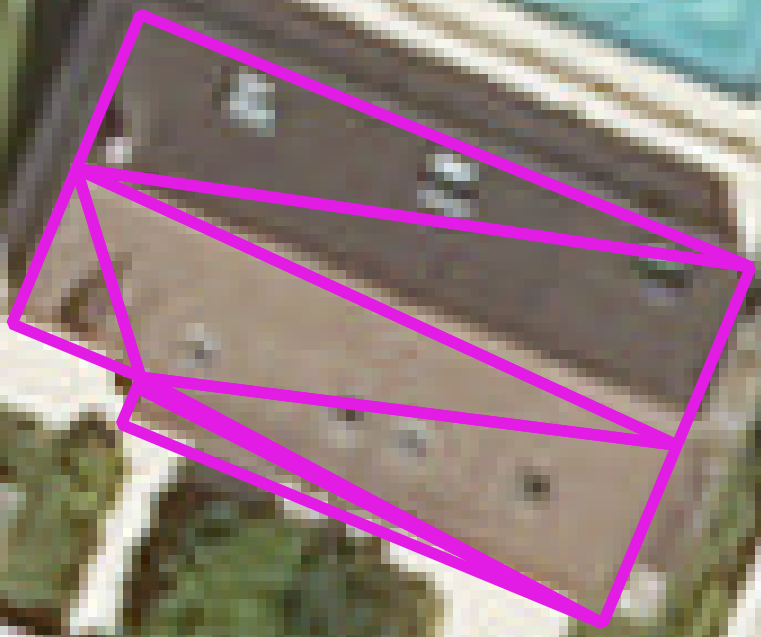
\includegraphics[height=.65\textwidth]{images/errors/facet/border}}
                                \caption{\label{fig::fac_footprint} Imprecise borders}
                            \end{subfigure}
                            \begin{subfigure}{.45\textwidth}
                                \centering
                                \fbox{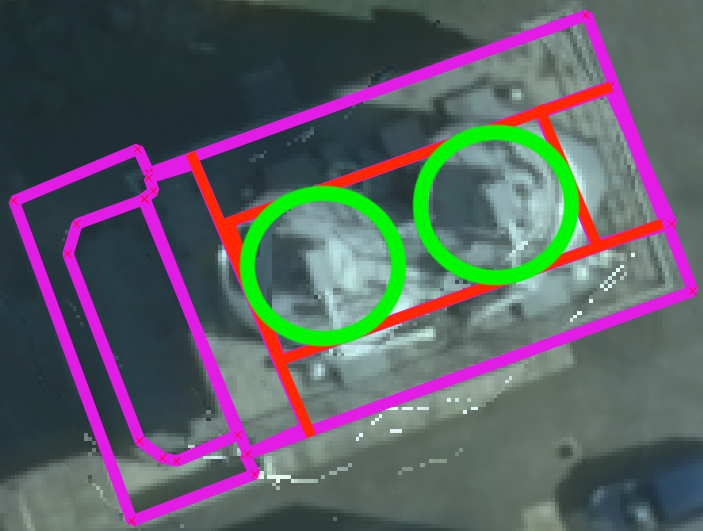
\includegraphics[height=.65\textwidth]{images/errors/facet/topology}}
                                \caption{\label{fig::fac_height} Inaccurate topology}
                            \end{subfigure}
                        \end{center}
                    \end{figure}
                }
            \end{frame}
        \subsection{Quality prediction pipeline}
            \begin{frame}{The evaluation pipeline}
                \begin{figure}
                    \includestandalone[mode=buildnew, width=\textwidth]{graphical_abstract}
                \end{figure}
            \end{frame}
            \begin{frame}{Geometric features}
                \begin{figure}
                    \includestandalone[mode=buildnew, height=.75\textheight]{geometric_features}
                \end{figure}
            \end{frame}
            \begin{frame}{Height-based features}
                \begin{figure}
                    \includestandalone[mode=buildnew, width=\textwidth]{altimetric_features}
                \end{figure}
            \end{frame}
            \begin{frame}{Image-based features}
                \begin{figure}
                    \begin{subfigure}{.48\textwidth}
                        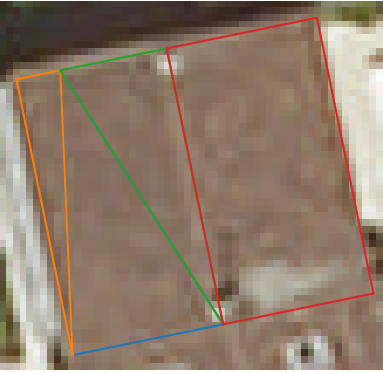
\includegraphics[width=.9\textwidth]{images/radio_vector}
                        \caption{\label{fig::ortho_sup} Building nadir projection on an orthoimage.}
                    \end{subfigure}
                    \begin{subfigure}{.48\textwidth}
                        \includestandalone[mode=buildnew, width=.9\textwidth]{radiometric_features}
                        \caption{\label{fig::hist} cosine \underline{similarity} between facet edge normal \textcolor{blue}{$\vec n$} and image gradient \textcolor{purple}{$\vec \nabla I$} for each \textcolor{green}{intersecting} pixel.}
                    \end{subfigure}
                \end{figure}
            \end{frame}
    \section{Experiments}
        \begin{frame}{Datasets}
            \begin{table}
                \begin{center}
                    \scriptsize
                    \begin{tabular}{c c c c}
                        \toprule
                        & \textbf{Elancourt} & \textbf{Nantes} & \textbf{Paris-13} \\
                        \midrule
                        \# samples & 2009 & 748 & 478 \\
                        DSM res. & \SI{6}{\cm} & \SI{10}{\cm} & \SI{10}{\cm} \\
                        Img. res. & \SI{6}{\cm} & \SI{10}{\cm} & \SI{10}{\cm} \\
                        Typology & bi-level + flat roof & dense city center & Haussmann style + high towers \\
                        \bottomrule
                    \end{tabular}
                    \caption{Dataset details.}
                \end{center}
            \end{table}
            \uncover<2->{
                \begin{table}
                    \begin{center}
                        \scriptsize
                        \begin{tabular}{c c c}
                            \toprule
                            Geometric & Height based & Image based \\
                            \midrule
                            $\approx$ \SI{0.05}{\second}/building & $\approx$ \SI{1.4}{\second}/building & $>$ \SI{16}{\second}/building \\
                            \bottomrule
                        \end{tabular}
                        \caption{Running time per feature type.}
                    \end{center}
                \end{table}
            }
        \end{frame}
        \begin{frame}{Ablation study: Elancourt example}
            \begin{table}
                \scriptsize
                \begin{center}
                    \scriptsize
                    \begin{tabular}{|x{.7cm} | x{.8cm} x{.8cm} | x{.8cm} x{.8cm} | x{.8cm} x{.8cm} | x{.8cm} x{.8cm}|}
                        \hline
                        &\multicolumn{2}{x{1.6cm}|}{\textbf{Geom.}} & \multicolumn{2}{x{1.6cm}|}{\textbf{Geom. $\cup$ Hei.}} & \multicolumn{2}{x{1.6cm}|}{\textbf{Geom. $\cup$ Im.}} & \multicolumn{2}{x{1.6cm}|}{\textbf{All}}\\
                        \cline{2-9}
                        &\textbf{Rec.} & \textbf{Prec.} & \textbf{Rec.} & \textbf{Prec.} & \textbf{Rec.} & \textbf{Prec.} & \textbf{Rec.} & \textbf{Prec.}\\
                        \hline
                        \texttt{BOS} & \textbf{93.96} & 76.15 & 91.43 & \textbf{77.76} & 91.51 & 76.08 & 90.83 & 76.14 \\
                        \hline
                        \texttt{BUS} & 32.98 & \textbf{76.47} & \textbf{41.86} & 75.57 & 40.38 & 71.00 & 39.32 & 71.81 \\
                        \hline
                        \texttt{BIB} & 12.32 & 67.57 & 12.81 & \textbf{68.42} & 16.26 & 67.35 & \textbf{16.75} & 68.0 \\
                        \hline
                        \texttt{BIT} & \textbf{25.25} & 92.59 & 20.20 & 90.91 & 20.20 & \textbf{95.24} & 11.11 & 91.67 \\
                        \hline
                        \hline
                        \texttt{FOS} & 98.91 & 99.07 & 98.91 & \textbf{99.30} & \textbf{98.99} & 98.84 & 98.91 & 98.84 \\
                        \hline
                        \texttt{FUS} & \textbf{1.90} & 54.55 & 0.63 & \textbf{66.67} & 1.61 & 50 & 1.27 & \textbf{66.67} \\
                        \hline
                        \texttt{FIB} & \textbf{9.17} & 87.5 & 0 & --- & 8.30 & 82.61 & 7.42 & \textbf{100} \\
                        \hline
                        \texttt{FIT} & \textbf{6.67} & \textbf{100} & 8.73 & 95.24 & 3.33 & \textbf{100} & 3.33 & \textbf{100} \\
                        \hline
                        \texttt{FIG} & \textbf{80.54} & 73.14 & 80.45 & \textbf{72.62} & 78.69 & 72.12 & 79.02 & 71.82 \\
                        \hline
                    \end{tabular}
                \end{center}
            \end{table}
        \end{frame}
        \begin{frame}{Scalability study: possible experimentations}
            \begin{figure}
                \includestandalone[mode=buildnew, height=.7\textheight]{scalabitity_graph}
            \end{figure}
        \end{frame}
        \begin{frame}{Transferability and Generalization of predictions}
            \begin{table}
                \scriptsize
                \begin{center}
                    \begin{tabular}{c c| x{.4cm} x{.4cm} x{.4cm} x{.4cm} |x{.4cm} x{.4cm} x{.4cm} x{.55cm} x{.4cm}}
                        \hline
                        &&\texttt{BOS}  & \texttt{BUS} &\texttt{BIB} &\texttt{BIT} &\texttt{FOS}  & \texttt{FUS} &\texttt{FIB} &\texttt{FIT} &\texttt{FIG} \\
                        \hline
                        \multirow{6}{*}{\rotatebox{90}{Transf.}}&El. $\rightarrow$ Na. &\cellcolor{Moins1} & \cellcolor{Moins2}&\cellcolor{Moins1}& \cellcolor{Moins2}& \cellcolor{Zero}& \cellcolor{Zero}&\cellcolor{Plus2} Im. & \cellcolor{Moins1}&\cellcolor{Zero}\\
                        &El. $\rightarrow$ P-13  & \cellcolor{Moins1}& \cellcolor{Moins2}& \cellcolor{Zero}& \cellcolor{Moins2}& \cellcolor{Zero}& \cellcolor{Plus1}Im.& \cellcolor{Plus1}Im.& \cellcolor{Moins1}&\cellcolor{Zero}\\
                        &Na. $\rightarrow$ P-13  & \cellcolor{Moins1}& \cellcolor{Moins2}& \cellcolor{black} & \cellcolor{Plus2}& \cellcolor{Zero}& \cellcolor{Plus1}& \cellcolor{Plus1}& \cellcolor{black} &\cellcolor{Zero}\\
                        &Na. $\rightarrow$ El.  &\cellcolor{Plus1} & \cellcolor{Moins1}& \cellcolor{Moins1}&\cellcolor{Plus1}All & \cellcolor{Zero}& \cellcolor{Moins2}&\cellcolor{Moins1}Im. &\cellcolor{Plus1}Im. &\cellcolor{Zero}\\
                        &P-13 $\rightarrow$ Na.  &\cellcolor{Moins2} & \cellcolor{Moins1}& \cellcolor{black} & \cellcolor{Plus1}&\cellcolor{Zero} & \cellcolor{Moins3}& \cellcolor{Zero}& \cellcolor{black} & \cellcolor{Moins1} Hei.\\
                        &P-13 $\rightarrow$ El. &\cellcolor{Zero} &\cellcolor{Moins1} & \cellcolor{Plus1}Im. & \cellcolor{Zero}& \cellcolor{Zero}& \cellcolor{Moins4}& \cellcolor{Moins2}Im. & \cellcolor{black} & \cellcolor{Zero}\\
                        \hline
                        \multirow{3}{*}{\rotatebox{90}{General.}  }&El.   & \cellcolor{Moins2}& \cellcolor{Moins2}Im.& \cellcolor{Moins2}&\cellcolor{Moins2} &\cellcolor{Zero} &\cellcolor{Plus1}Im. &\cellcolor{Plus2}Im. &\cellcolor{Moins1}Geom. & \cellcolor{Moins1} Hei\\
                        &Na.   & \cellcolor{Zero}All& \cellcolor{Moins2}Im.&\cellcolor{Moins1}Im. &\cellcolor{Plus2} &\cellcolor{Zero} & \cellcolor{Zero}& \cellcolor{Moins2}Im.& \cellcolor{black} &\cellcolor{Zero}\\
                        &P-13   &\cellcolor{Moins2}All &\cellcolor{Moins2} & \cellcolor{black} &\cellcolor{Plus1}Hei. &\cellcolor{Zero} &\cellcolor{Moins4} &\cellcolor{Moins2}Im. & &\cellcolor{Moins1}\\
                        \hline
                    \end{tabular}
                    \caption{The color indicates the change magnitude: \textcolor{Moins4}{$\blacksquare$}: $[-45,-35\%[$-- \textcolor{Moins3}{$\blacksquare$}: $[-35,-25\%[$ -- \textcolor{Moins2}{$\blacksquare$}: $[-25,15\%[$-- \textcolor{Moins1}{$\blacksquare$}: $[-15, 5\%[$ -- $\square$: $[-5,5\%[$-- \textcolor{Plus1}{$\blacksquare$}: $[5,15\%[$ -- \textcolor{Plus2}{$\blacksquare$}: $[15,25\%]$ -- $\blacksquare$: cannot be computed.}
                \end{center}
            \end{table}
        \end{frame}
        \begin{frame}{Representativeness study: F-score stability}
            \begin{figure}
                \includestandalone[mode=buildnew, height=.7\textheight]{f-scores_f3_repr}
            \end{figure}
        \end{frame}
        \begin{frame}{Some failure cases on Elancourt}
            \begin{figure}
                \begin{center}
                \tiny
                    \begin{tabular}{| x{.06\textwidth} | x{.035\textwidth} | x{.035\textwidth} || x{.06\textwidth} | x{.035\textwidth} | x{.035\textwidth} || x{.06\textwidth} | x{.035\textwidth} | x{.035\textwidth} || x{.06\textwidth} | x{.035\textwidth} | x{.035\textwidth} |}
                        \hline
                        \multicolumn{3}{| c ||}{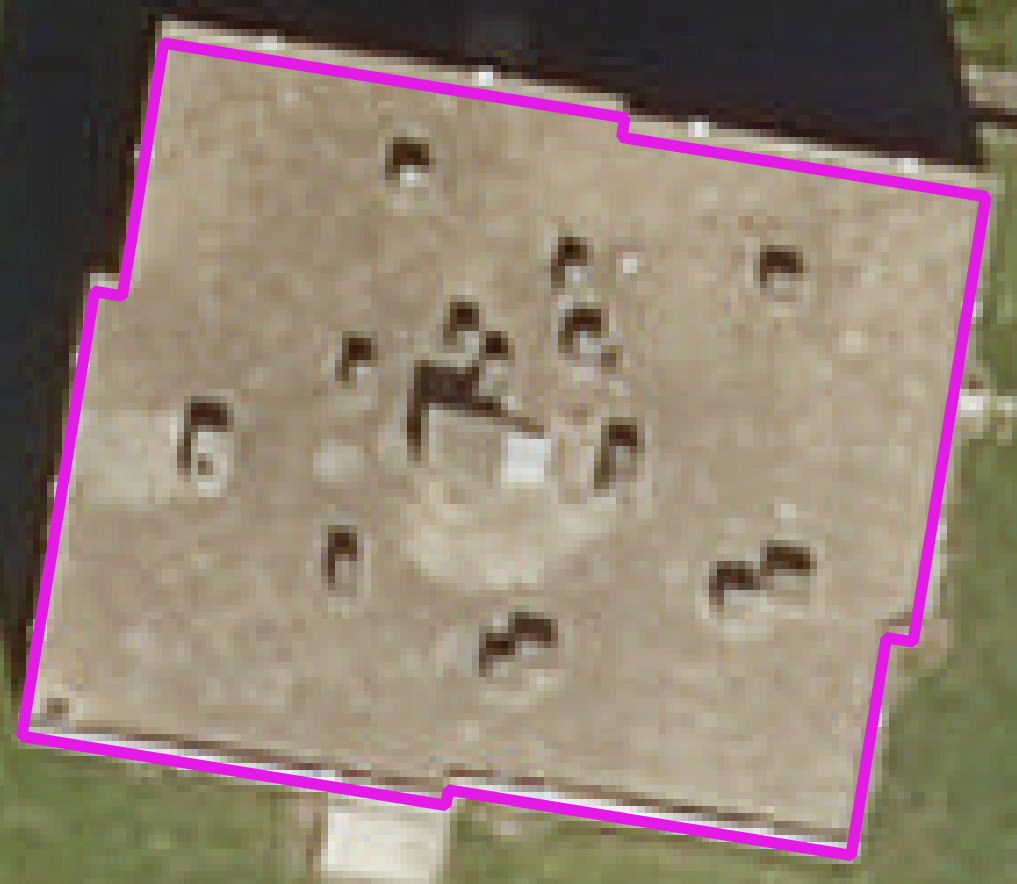
\includegraphics[width=.2\textwidth,valign=m,margin=1pt 1pt]{images/prediction_results/valid_as_bul_over}} & \multicolumn{3}{ c ||}{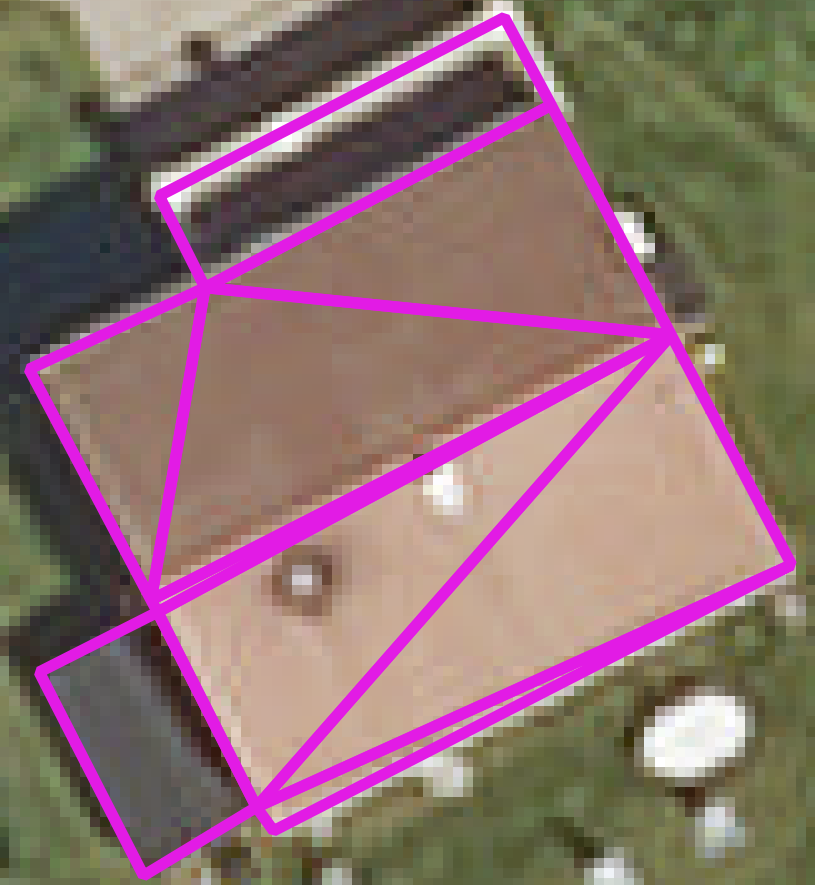
\includegraphics[width=.2\textwidth,valign=m,margin=0cm 1pt]{images/prediction_results/no_imprec_no_fac_over}} & \multicolumn{3}{ c ||}{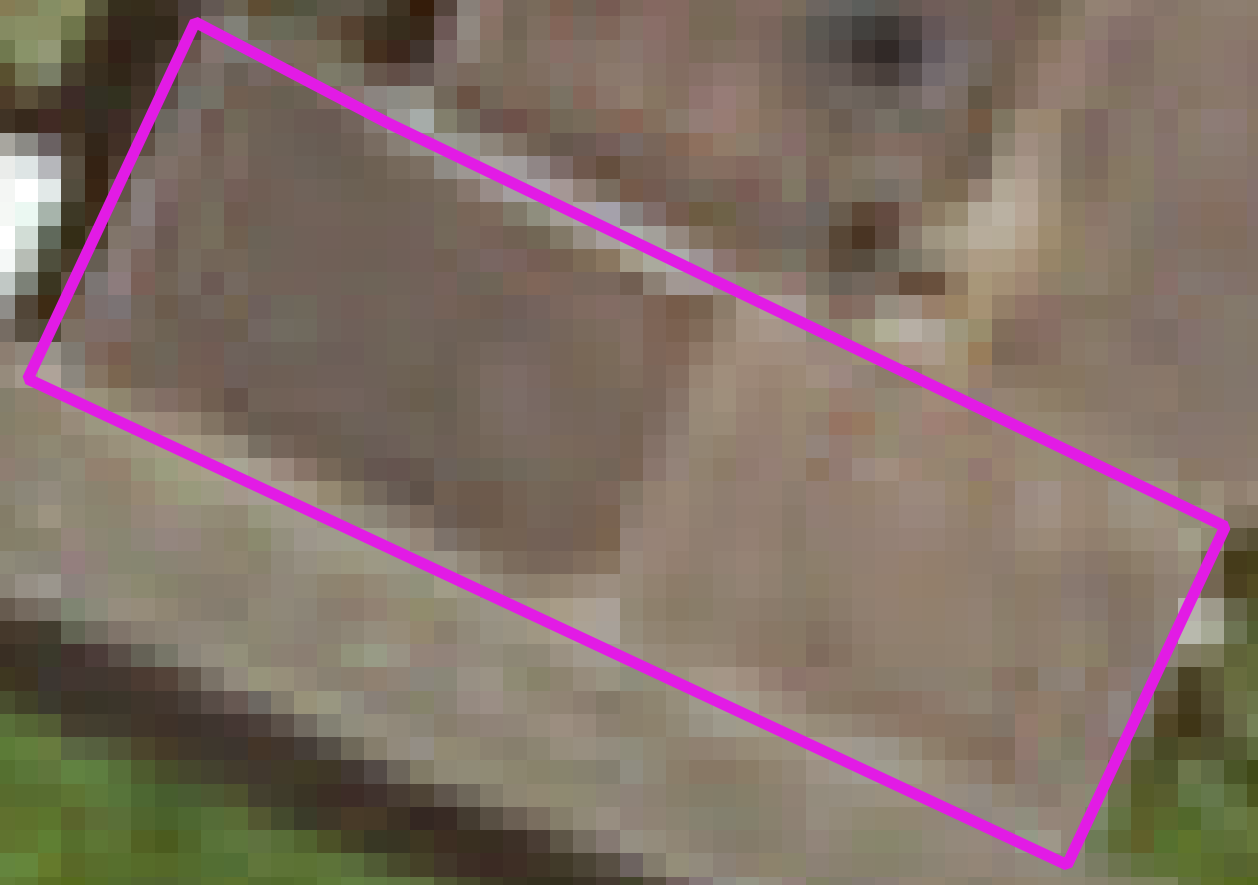
\includegraphics[width=.2\textwidth,valign=m,margin=0cm 1pt]{images/prediction_results/no_under_seg}} & \multicolumn{3}{ c |}{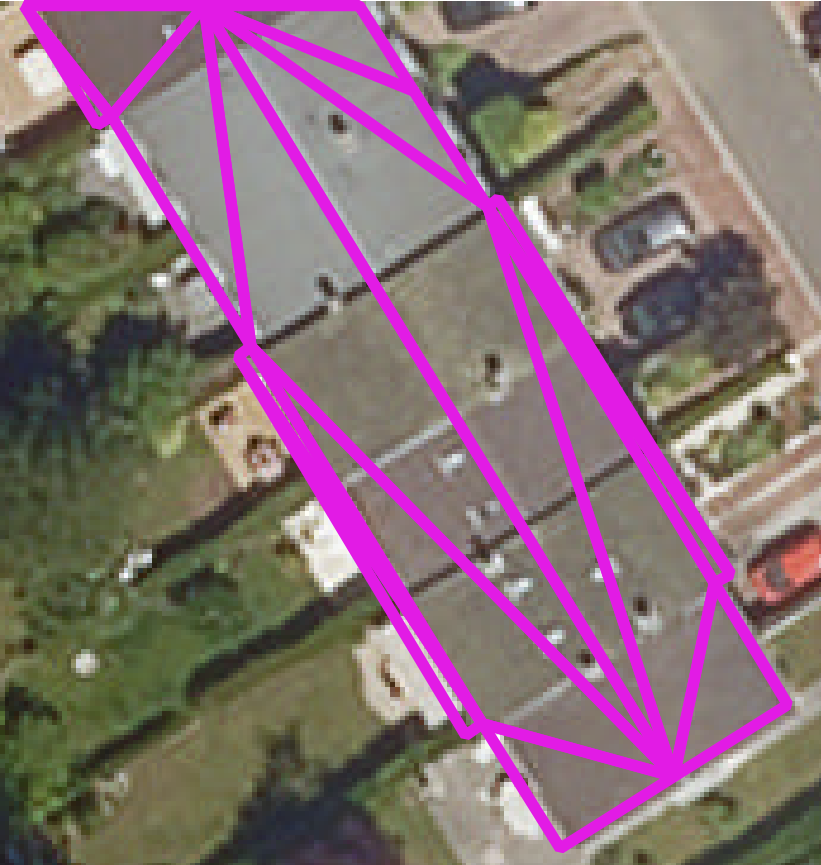
\includegraphics[width=.2\textwidth,valign=m,margin=0cm 1pt]{images/prediction_results/no_bul_under_seg}} \\
                        \hline
                        \textbf{Errors} & \textbf{G.T.} & \textbf{Pred.} & \textbf{Errors} & \textbf{G.T.} & \textbf{Pred.} & \textbf{Errors} & \textbf{G.T.} & \textbf{Pred.} & \textbf{Errors} & \textbf{G.T.} & \textbf{Pred.}\\
                        \hline
                        \texttt{BOS} & \xmark & \cmark & \texttt{BUS} & \xmark & \cmark & \texttt{BOS} & \cmark & \cmark & \texttt{BOS} & \cmark & \xmark \\
                         &  &  & \texttt{FIG} & \cmark & \xmark & \texttt{FUS} & \cmark & \xmark &  \texttt{FOS} & \cmark & \xmark \\
                            &  &  & \texttt{FOS} & \cmark & \xmark &  &  &  & \texttt{BUS} & \cmark & \xmark \\
                            &  &  &  &  &  &  &  &  &  \texttt{BIB} & \cmark & \cmark \\
                        \hline
                    \end{tabular}
                \end{center}
            \end{figure}
        \end{frame}
        
    \section{Conclusion}
        \begin{frame}{\textcolor{yellow}{Conclusion} \& \textcolor{purple}{Perspectives}}
            \begin{itemize}[label=$\blacktriangleright$, font=\color{yellow}, itemsep=2em]
                \item \textbf{Flexible, robust and hierarchical} taxonomy;
                \item \textbf{Fast, lightweight and modular} pipeline for model evaluation;
                \item Baseline for geometric, image-based and height-based features;
            \end{itemize}
            \uncover<2->{
                ~\\
                Future work:
                \begin{itemize}[label=$\blacktriangleright$, font=\color{purple}, itemsep=2em]
                    \item Dataset augmentation $\longrightarrow$ \textbf{Simulate errors} from the taxonomy based on reference data;
                    \item Extend to richer features $\longrightarrow$ Graph kernels, deep learning.
                \end{itemize}
            }
        \end{frame}
    \section{References}
        \begin{frame}[allowframebreaks]{References}
            \printbibliography
        \end{frame}
\end{document}